\subsection{Jacobi}

\begin{frame}
		\frametitle{\textbf{3. Iterative methods}}
	
	
	    \visible<1->{
		\begin{shaded}
			\textbf{Goal of all iterative methods}
			\begin{itemize}
			\item Goal is to annhilate some components of teh residual vector $r=b-\mathcal{A}x$
			\item We will try to find a solution for $x$ that satisfies $\lVert x \rVert < \mathrm{tol}$
			\end{itemize}
	\end{shaded}}
		
    \visible<2->{
	\begin{shaded}
		\textbf{Jacobi's method}
		\begin{itemize}
			\item Simplest method to solve a linear system. Slow and has some stringent convergence properties.
		\end{itemize}
\end{shaded}}
\end{frame}

\begin{frame} 
\frametitle{\textbf{3. Jacobi's method component form}}

In what follows, $\xi_i^{(k)}$ denotes the ith component of the iterate $x_k$. In the same way, $\beta_i$ will be the ith component of the right-hand side $b$. $a_{ij}$ is the ijth component of $\mathcal{A}$.

Jacobi's method consists in solving:
\[
a_{ij} \xi_i^{k+1} = - \sum_{j=1,i\neq j}^n a_{ij} \xi_j^{(k)} + \beta_i
\]

Which results in:
\[
 \xi_i^{k+1} = \frac{1}{a_{ij}} \left( - \sum_{j=1,i\neq j}^n a_{ij} \xi_j^{(k)} + \beta_i \right)
\]

\end{frame}

\begin{frame} 
	\frametitle{\textbf{3. Jacobi's method matrix form}}
	
	We begin with the decomposition:
	\[
	\mathcal{A} = \mathcal{D} - \mathcal{E}-\mathcal{F}
	\]
	
	where $\mathcal{D}$ is the diagonal, $\mathcal{E}$ is the strict lower part and $\mathcal{F}$ is the strict upper part. A Jacobi iteration is equivalent to:
	
	\[
	x^{k+1} = \mathcal{D}^{-1} (\mathcal{E} + \mathcal{F})x^{k} + \mathcal{D}^{-1} b
	\]
\end{frame}

\begin{frame}
\frametitle{\textbf{3. Jacobi's resuls}}
	
\begin{center}
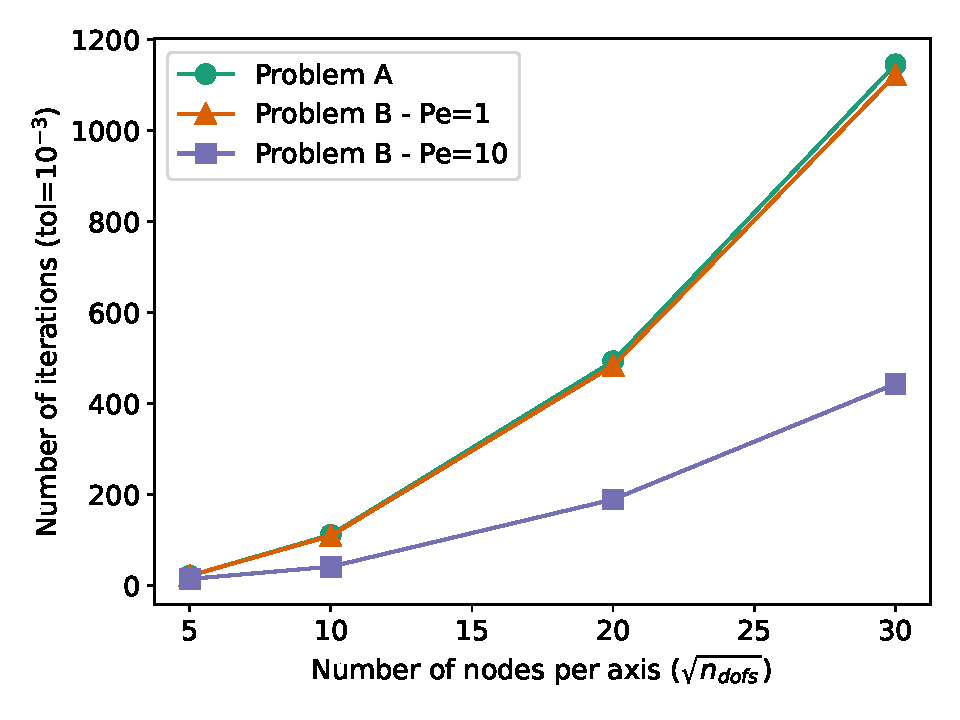
\includegraphics[width=0.95\linewidth]{images/j_its}
\end{center}
\end{frame}

\subsection{Gauss Seidel}
\begin{frame} 
	\frametitle{\textbf{3. Gauss Seidel's method component form}}
	
	Gauss Seidel's method consists in solving:
	\[
	a_{ij} \xi_i^{k+1} = - \sum_{j=1}^{i-1} a_{ij} \xi_j^{(k+1)} - \sum_{j=i+1}^n a_{ij} \xi_j^{(k)} + \beta_i
	\]
	
Which results in:
\[
\xi_i^{k+1} = \frac{1}{a_{ij}} \left( - \sum_{j=1}^{i-1} a_{ij} \xi_j^{(k+1)} - \sum_{j=i+1}^n a_{ij} \xi_j^{(k)} + \beta_i \right)
\]
	
\end{frame}

\begin{frame} 
	\frametitle{\textbf{3. Gauss Seidel's method matrix form}}
	
	We continue with the decomposition:
	\[
	\mathcal{A} = \mathcal{D} - \mathcal{E}-\mathcal{F}
	\]
	
	where $\mathcal{D}$ is the diagonal, $\mathcal{E}$ is the strict lower part and $\mathcal{F}$ is the strict upper part. A Gauss Seidel iteration is equivalent to:
	
	\[
	x^{k+1} = \left(\mathcal{D}-\mathcal{E}\right)^{-1}\mathcal{F}x^{k} +  \left(\mathcal{D}-\mathcal{E}\right)^{-1} b
	\]
	
\end{frame}

\begin{frame}
	\frametitle{\textbf{3. Gauss Seidel results}}
	\centering
	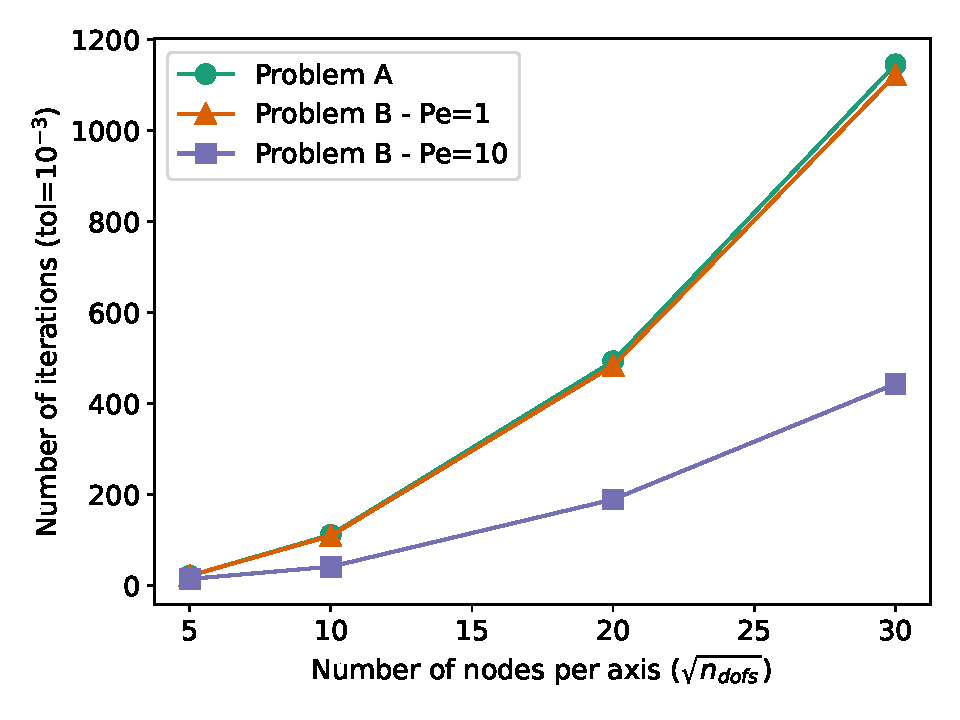
\includegraphics[width=0.95\linewidth]{images/j_its}
\end{frame}

\subsection{Convergence}

\begin{frame}
\frametitle{\textbf{3. Convergence}}

All methods we have seen define a recurrence (or series of iterate):
\[
x^{k+1} = \mathcal{G} x^k + f
\]

Where $\mathcal{G}$ is an \textit{iteration matrix}.

    \visible<1->{
	\begin{shaded}
		\textbf{Three things we need (but won't prove)}
		\begin{enumerate}[label=\Alph*]
\item If the iterations converge, this we converge to the right solution?
\item Under which condition does the iteration converge?
\item When the iteration converge, how fast does it?
		\end{enumerate}
\end{shaded}}
\end{frame}

\begin{frame}
	\frametitle{\textbf{3. Theorem}}

\begin{shaded}
	\textbf{General convergence theorem}
	\begin{itemize}
		\item If $\mathcal{I}-\mathcal{G}$ is non-singular and $\rho(\mathcal{G})<1$ then the method converges for every $f$ and $x_0$.
		\item The convergence rate $\tau$ is the natural logarithm of the inverse of the convergence factor which is the spectral radius:
		\[
		\tau = - \ln \left(\rho\right)
		\]
	\end{itemize}
	
		
\end{shaded}

   \visible<2->{
\begin{shaded}
\textbf{But what is the spectral radius $\rho(\mathcal{G})<1$?}
\begin{itemize}
\item It is the spectral radius of a square matrix is the maximum of the absolute values of its eigenvalues.
\end{itemize}
\end{shaded}}

\visible<3->{
\begin{shaded}
\textbf{What did we get for our $25\times25$ case?}
\begin{itemize}
\item Jacobi : $\rho=0.991$
\item Gauss-Seidel : $\rho=0.983$
\end{itemize}
\end{shaded}}
		
	

\end{frame}
